\chapter{Implementacija i korisničko sučelje}
		
		
		\section{Korištene tehnologije i alati}
		
			Komunikacija u timu odvijala se videopozivima putem aplikacije \underline{\href{https://www.microsoft.com/en-us/microsoft-teams/group-chat-software}{Microsoft Teams}}\textsuperscript{1}. Za izradu UML dijagrama korišteni su alati \underline{\href{https://astah.net/products/astah-uml/}{Astah UML}}\textsuperscript{2} i \underline{\href{https://online.visual-paradigm.com/}{Visual Paradigm}}\textsuperscript{3}. \underline{\href{https://git-scm.com/}{Git}}\textsuperscript{4} je korišten kao sustav za upravljanje kodom. Projekt je dostupan na web platformi \underline{\href{https://github.com/}{GitHub}}\textsuperscript{5}
			
			\indent Za razvoj aplikacije korištena su razvojna okruženja \underline{\href{https://www.jetbrains.com/idea/}{IntelliJ IDE}}\textsuperscript{6} i \newline\underline{\href{https://code.visualstudio.com/}{Visual Studio Code}}\textsuperscript{7}. IntelliJ jedano je od najpopularnijih razvojnih okruženja za razvoj aplikacija u programskom jeziku Java. Izgradila ga je tvrtka JetBrains. Pruža bogatu podršku za razvoj desktop i web aplikacija. Visual Studio Code je također vrlo popularan uređivač za pisanje programskog koda, osobita za razvoj frontend dijela aplikacija jer pruža izrazito dobru podršku za frotend radne okvire. On je pod vlasištvom tvrtke Microsoft.
			
			\indent Aplikacija je napisana koristeći radni okvir \underline{\href{https://spring.io/projects/spring-boot/}{Spring Boot}}\textsuperscript{8} i jezik \underline{\href{https://www.oracle.com/java/}{Java}}\textsuperscript{9} za izradu \textit{backenda} te \underline{\href{https://react.dev/}{React}}\textsuperscript{10} i jezik \underline{\href{https://www.javascript.com/}{JavaScript}}\textsuperscript{11} za izradu \textit{frontenda}. React je bilioteka izražena u JavaScriptu koja olakšava izradu korisničkog sučelja. React je održava tvrtka Meta. Radni okvir Spring Boot nadograđuje mogućnosti samog programskog jezika Java te time uvelike olakšava razvoj web aplikacija. Nudi niz gotovih funkcionalnosti koji povećavaju produktivnost i efikasnost programera.
			
			\indent Za bazu podataka korišten je \underline{\href{https://www.postgresql.org/}{PostgreSQL}}\textsuperscript{12}.
			\noindent\\[1ex]\rule{0.5\linewidth}{0.5pt}\newline
			\noindent\textsuperscript{1}\url{https://www.microsoft.com/en-us/microsoft-teams/group-chat-software}\newline
			\noindent\textsuperscript{2}\url{https://astah.net/products/astah-uml/}\newline
			\noindent\textsuperscript{3}\url{https://online.visual-paradigm.com/}\newline
			\noindent\textsuperscript{4}\url{https://git-scm.com/}\newline
			\noindent\textsuperscript{5}\url{https://github.com/}\newline
			\noindent\textsuperscript{6}\url{https://www.jetbrains.com/idea/}\newline
			\noindent\textsuperscript{7}\url{https://code.visualstudio.com/}\newline
			\noindent\textsuperscript{8}\url{https://spring.io/projects/spring-boot/}\newline
			\noindent\textsuperscript{9}\url{https://www.oracle.com/java/}\newline
			\noindent\textsuperscript{10}\url{https://react.dev/}\newline
			\noindent\textsuperscript{11}\url{https://www.javascript.com/}\newline
			\noindent\textsuperscript{12}\url{https://www.postgresql.org/}\newline
			
		\newpage
		
		\section{Ispitivanje programskog rješenja}
			
			\indent Za provođenje testiranja naše Spring Boot aplikacije koristili smo biblioteke JUnit i Mockito. One su nam omogućile pouzdano i sustavno testiranje raličitih dijelova aplikacije. Za ispitivanje sustava koristili smo alat Selenium.
			 
	
			
			\subsection{Ispitivanje komponenti}
			U nastavku ovog poglavlja, pronaći ćete detaljan opis šest odabranih ispitnih slučajeva koji obuhvaćaju redovne situacije, rubne uvjete te testiranje ponašanja sustava u situacijama iznimki. Uz opis ispitnih slučajeva, priložili smo i odgovarajući izvorni kôd svakog testa, kao i rezultate izvođenja ispita u razvojnom okruženju, što omogućuje transparentnost i preglednost provedenih ispitivanja.
			
			Prvi test koji smo odradili je dohvaćanje romobila preko njegovog identifikatora. U ovom smo testu testirali servisni sloj naše aplikacije te set test uredno proveo.
			\begin{figure}[h]
				\centering
				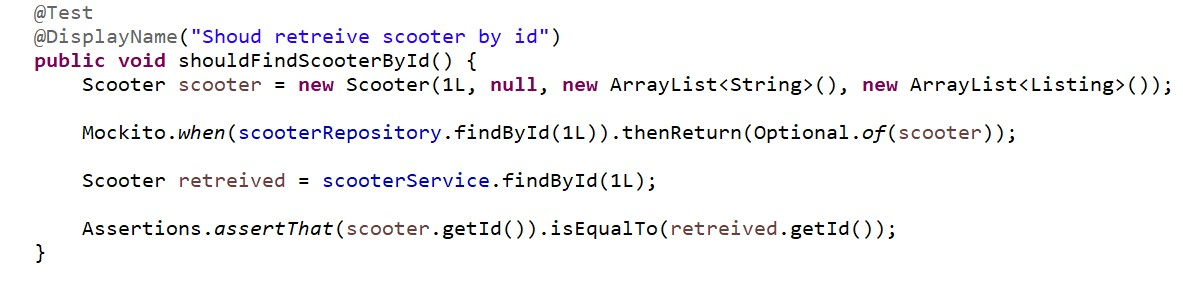
\includegraphics[width=0.6\textwidth]{slike/scooter_service_test.jpg}
				\caption{Testiranje dohvaćanja romobila preko identifikatora}
				\label{fig:Testiranje dohvaćanja romobila preko identifikatora}
			\end{figure}
			
			U sljedećem testu također smo testirali servisni sloj i to dohvaćanje poruka za dva korisnika. Dakle, u testu definiramo dva korisnika te provjeravamo vraća li nam naša aplikacija tražene poruke.
			\begin{figure}[h]
				\centering
				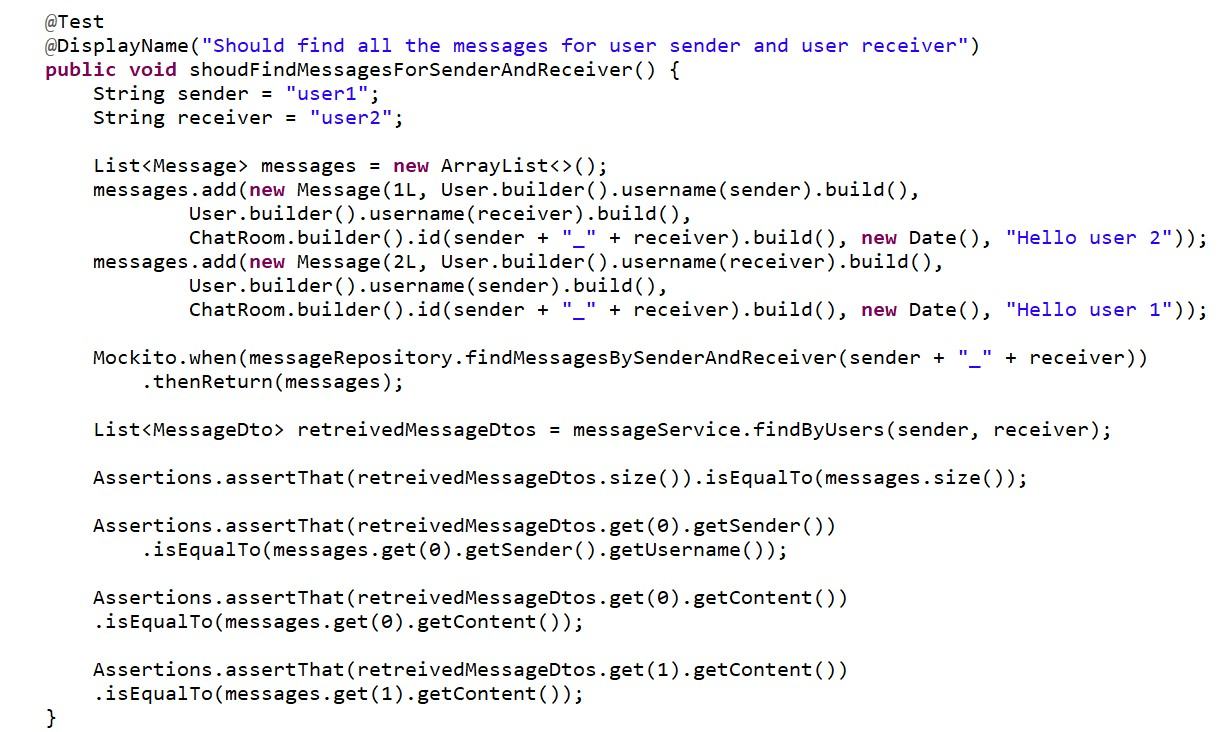
\includegraphics[width=0.6\textwidth]{slike/message_service_test.jpg}
				\caption{Testiranje dohvaćanja poruka za zadene korisnike}
				\label{fig:Testiranje dohvaćanja poruka za zadene korisnike}
			\end{figure}
			
			Sada ćemo prikazati testiranje ListingController. U prvom testu testirali smo dodavanje novog oglasa te je očekivani ishod odgovor poslužitelja sa novim oglasom, dok smo u drugom pokušali dohvatit oglas za nepostojeći romobil. U drugom testu očekuujemo da poslužitelj baci novu NullPointerException iznimku. Oba testa su se izvršila ispravno. \newline
			
			  \begin{figure}
					  	\centering
					  	\subfigure{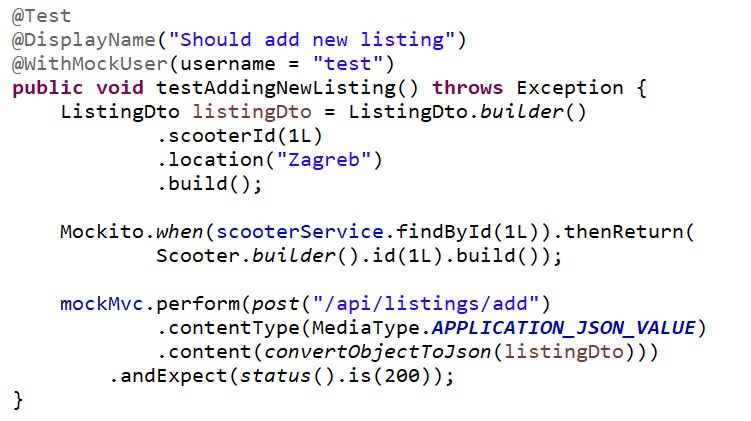
\includegraphics[width=0.4\textwidth]{slike/listing_controller_add_test.jpg}} 
					  	\subfigure{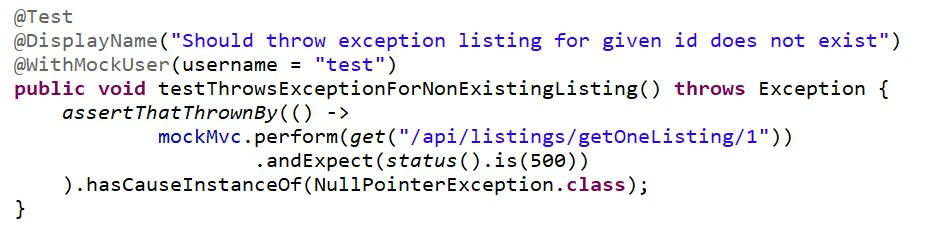
\includegraphics[width=0.4\textwidth]{slike/listing_controller_throw_test.jpg}} 
					  	\caption{Testiranje ListingController-a}
					  	\label{fig:Testiranje ListingController-a}
			  \end{figure}
			  
			Korisnik mora moći pregledavati romobile koje je trenutno iznajmio pa smo testirali i RentalController i to metodu koja osigurava dohvaćanje trenutnih najmova. U testu definiramo koje objekte tipa Rental očekujemo te kada primimo odgovor od poslužitelja provjeravamo jesmo li ih uistinu i primili. \newline
			
			\begin{figure}[h]
				\centering
				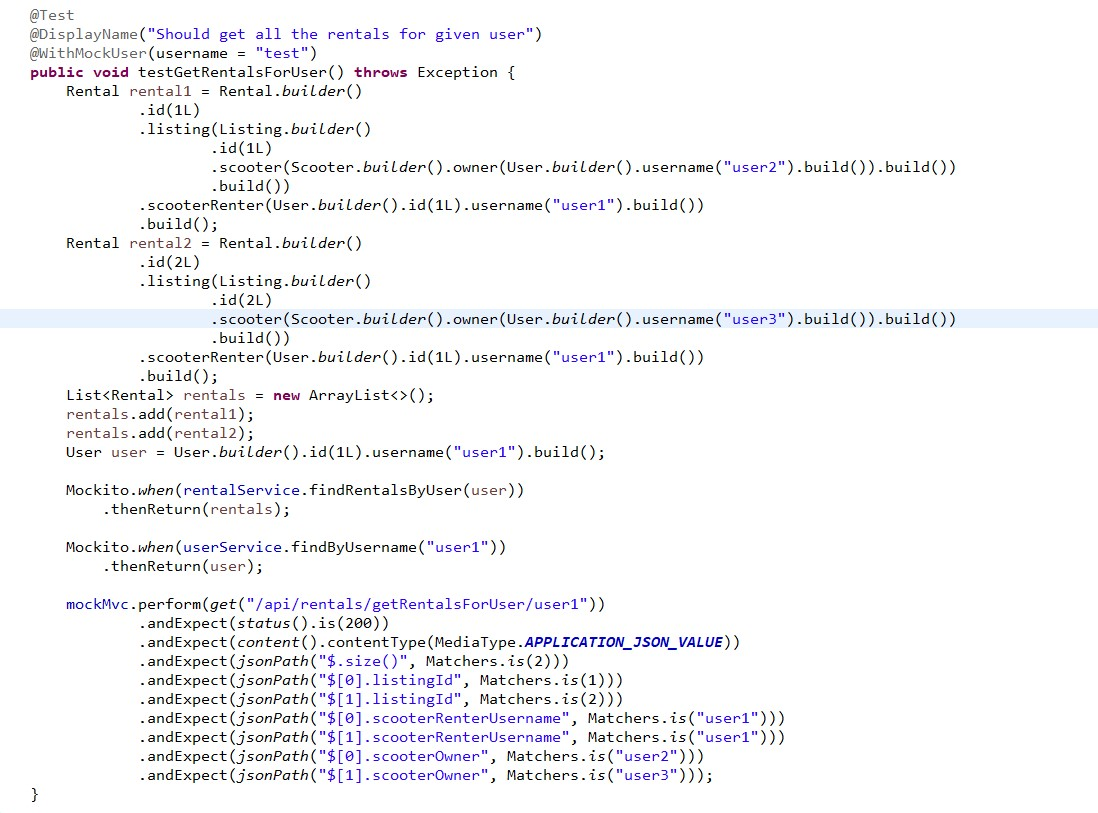
\includegraphics[width=0.6\textwidth]{slike/rental_controller_test.jpg}
				\caption{Testiranje dohvaćanja najmova za korisnika}
				\label{fig:Testiranje dohvaćanja najmova za korisnika}
			\end{figure}
			
			Na kraju, provjerili smo što će se dogodit ako pokušamo izbrisat ocjenu i komentar. Poslužitelj je prepoznao da ta funkcionalnost nije implementirana te ispravno odgovorio sa statusom 404 Not found.\newline
			
			\begin{figure}[h]
				\centering
				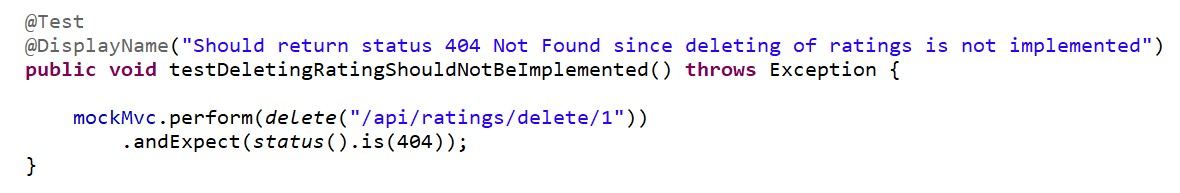
\includegraphics[width=0.6\textwidth]{slike/rating_controller_test.jpg}
				\caption{Testiranje brisanja komentara i ocjena}
				\label{fig:Testiranje brisanja komentara i ocjena}
			\end{figure}
			
			Sljedeća slika prikazuje da su se svi testovi uspješno proveli.
			\begin{figure}[h]
				\centering
				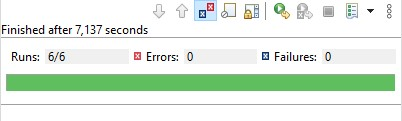
\includegraphics[width=0.6\textwidth]{slike/tests_passed.jpg}
				\caption{Uspješno provođenje testova}
				\label{fig:Uspješno provođenje testova}
			\end{figure}
			
			\subsection{Ispitivanje sustava}
			
			 \textit{Potrebno je provesti i opisati ispitivanje sustava koristeći radni okvir Selenium\footnote{\url{https://www.seleniumhq.org/}}. Razraditi \textbf{minimalno 4 ispitna slučaja} u kojima će se ispitati redovni slučajevi, rubni uvjeti te poziv funkcionalnosti koja nije implementirana/izaziva pogrešku kako bi se vidjelo na koji način sustav reagira kada nešto nije u potpunosti ostvareno. Ispitni slučaj se treba sastojati od ulaza (npr. korisničko ime i lozinka), očekivanog izlaza ili rezultata, koraka ispitivanja i dobivenog izlaza ili rezultata.\\ }
			 
			 \textit{Izradu ispitnih slučajeva pomoću radnog okvira Selenium moguće je provesti pomoću jednog od sljedeća dva alata:}
			 \begin{itemize}
			 	\item \textit{dodatak za preglednik \textbf{Selenium IDE} - snimanje korisnikovih akcija radi automatskog ponavljanja ispita	}
			 	\item \textit{\textbf{Selenium WebDriver} - podrška za pisanje ispita u jezicima Java, C\#, PHP koristeći posebno programsko sučelje.}
			 \end{itemize}
		 	\textit{Detalji o korištenju alata Selenium bit će prikazani na posebnom predavanju tijekom semestra.}
			
			\eject 
		
		
		\section{Dijagram razmještaja}
			
			\textbf{\textit{dio 2. revizije}}
			
			 \textit{Potrebno je umetnuti \textbf{specifikacijski} dijagram razmještaja i opisati ga. Moguće je umjesto specifikacijskog dijagrama razmještaja umetnuti dijagram razmještaja instanci, pod uvjetom da taj dijagram bolje opisuje neki važniji dio sustava.}
			
			\eject 
		
		\section{Upute za puštanje u pogon}
		\indent Našu aplikaciju odlučili smo pustit u pogon preko platformue Render. U ovom poglavlju objasnit ćemo korake koje smo proveli kako bi uspješno pustili u pogon aplikaciju.\newline
	
		\textbf{Konfiguracija baze podataka}\newline
		Na web stranici Render potrebno je odabrati izradu nove baze podataka te unijeti željeno ime baze te verziju PostgreSQL-a. Sljedeća slika prikazuje izradu baze podataka.
		\begin{figure}[h]
			\centering
			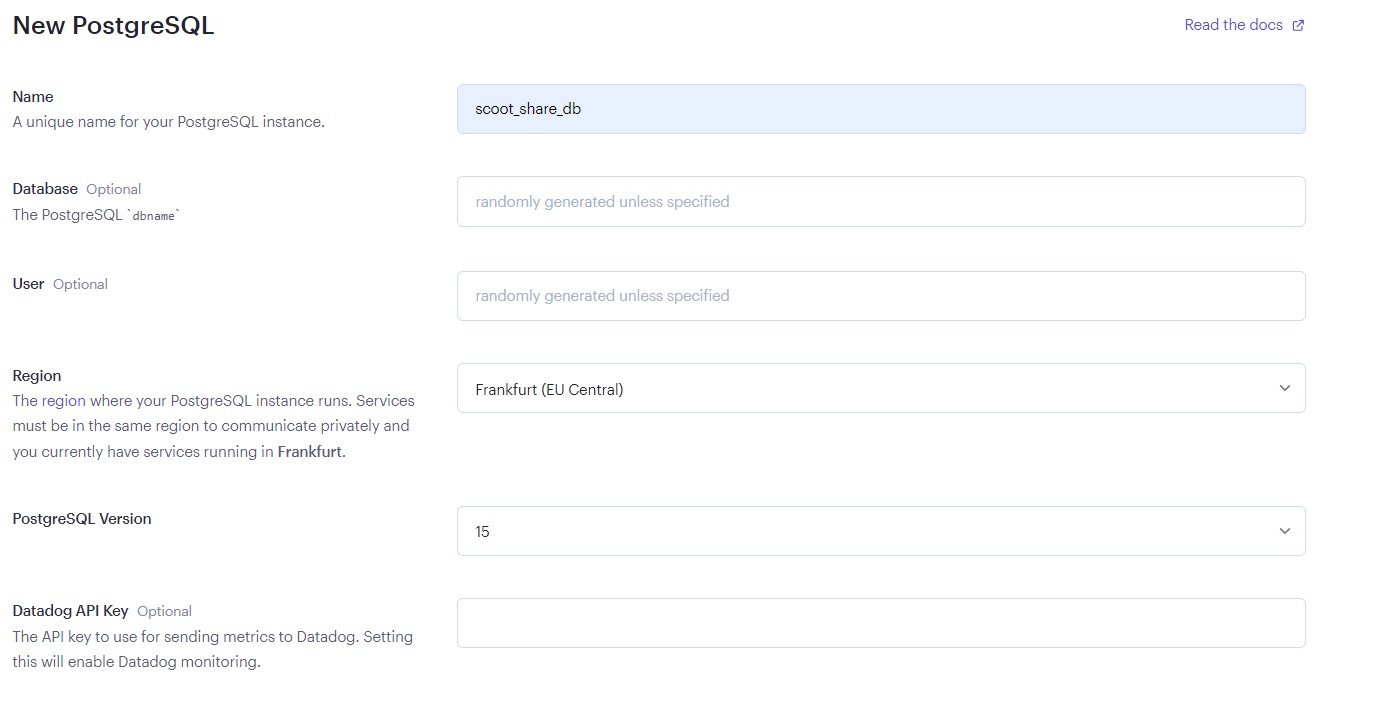
\includegraphics[width=0.8\textwidth]{slike/pustanju_u_pogon_1.jpg}
			\caption{Izrada baze podataka}
			\label{fig:baza podataka}
		\end{figure}
		
		
		\textbf{Konfiguracija backenda}\newline
		Kako bi mogli pustit u pogon našu poslužiteljsku stranu potrebno je učiniti određene izmjene. Potrebno je preurediti application.properties file na način da se dodaju globalne varijable koje će se koristit na Render-u. Također, treba dodati i Dockerfile koji sadrži niz instrukcija za izgradnju Docker kontejnera. 
		
		\begin{figure}
			\centering
			\subfigure{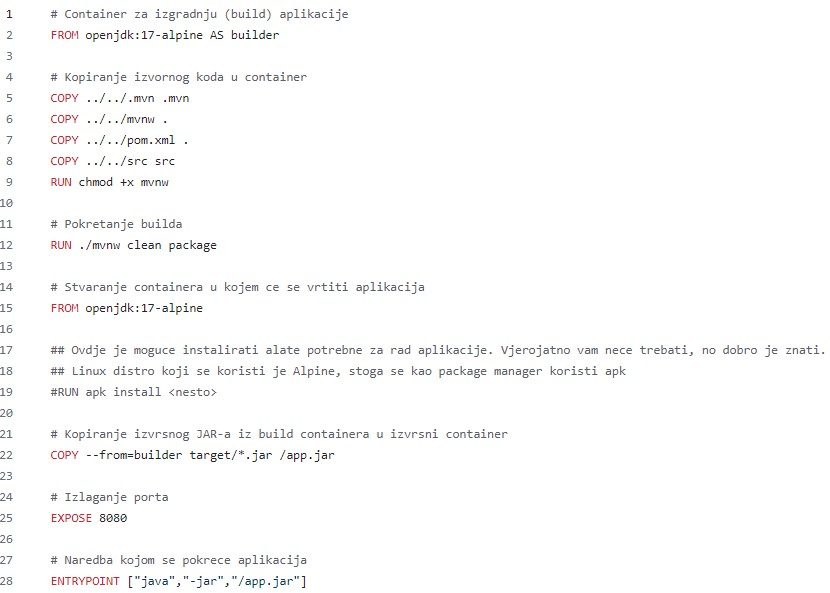
\includegraphics[width=0.24\textwidth]{slike/pustanju_u_pogon_2.jpg}} 
			\subfigure{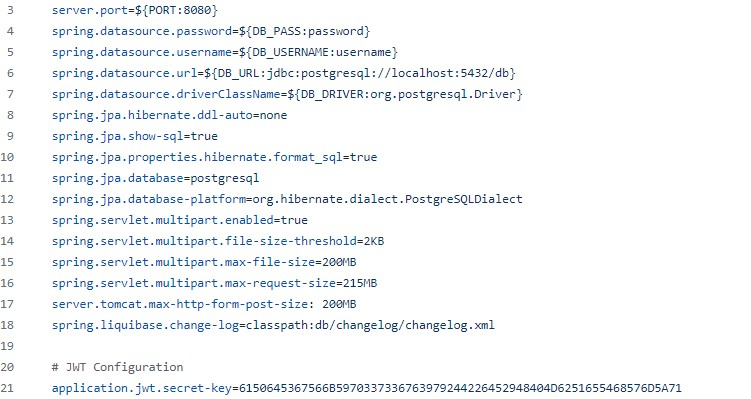
\includegraphics[width=0.24\textwidth]{slike/pustanju_u_pogon_3.jpg}} 
			\caption{Dockerfile i application.properties}
			\label{fig:dockerfile_application.properties}
		\end{figure}
		
		Nakon što je prvi korak odrađen potrebno je konfigurirati backend na Renderu. Odabiremo novi Web Service, nakon toga povežemo naš github repository s Renderom. 
		
		\begin{figure}[h]
			\centering
			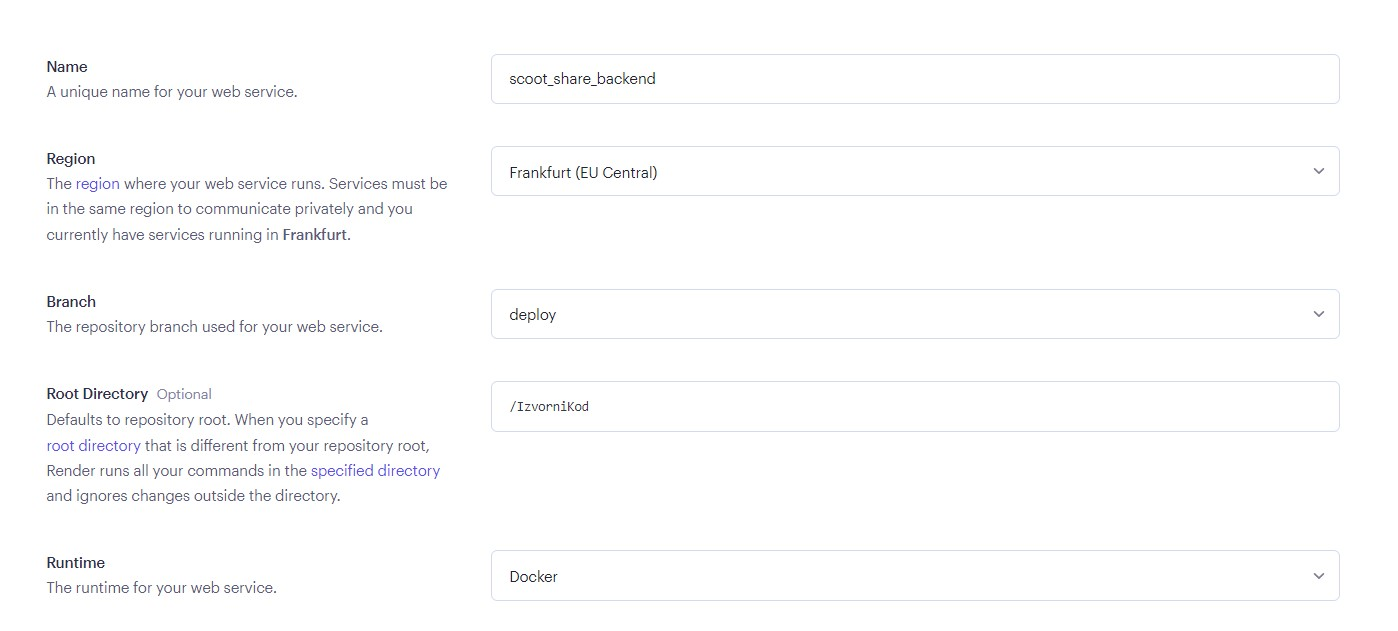
\includegraphics[width=0.8\textwidth]{slike/pustanju_u_pogon_4.jpg}
			\caption{Kreiranje backenda na Renderu}
			\label{fig:backend_render}
		\end{figure}
		
		\textbf{Konfiguracija frontenda}
		Potrebno je u našoj frontend React applikaciji u datoteci package.json dodati ovisnosti prema http-proxy-middleware, dotenv, express. Zatim treba dodati datoteku /src/setupProxy.js koja služi kao proxy server za lokalni development (redirecta api pozive na localhost:8080), odnosno kad se koristi react-scripts start skripta. Posljednja datoteka koju treba dodati je app.js u kojoj se nalazi express server za produkcijski proxy i posluzivanje frontenda. Jednom kada su sve izmjene napravljene i pohranjene u repozitorij kreirajmo Web Servis na Renderu za frontend. 
			
		\begin{figure}[h]
			\centering
			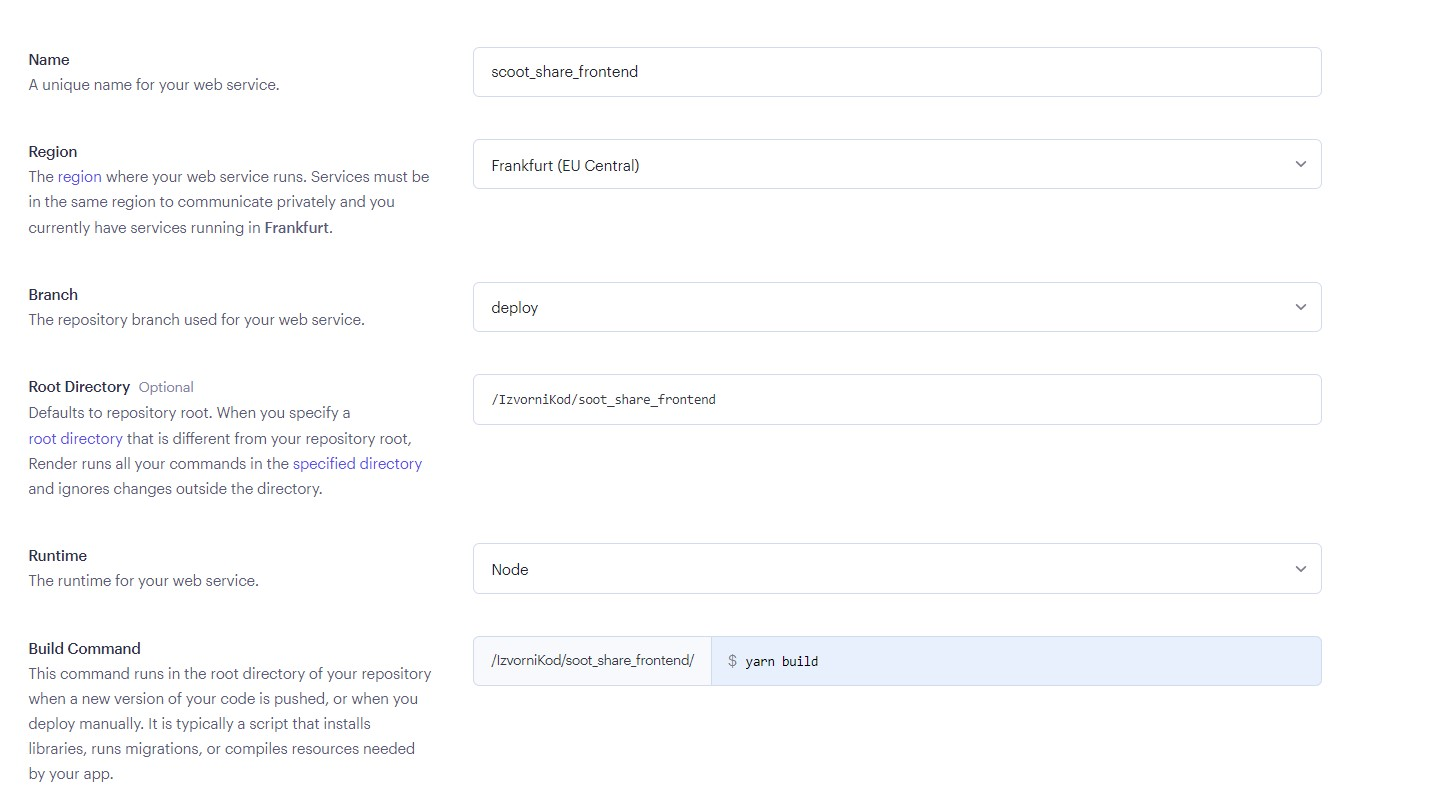
\includegraphics[width=0.8\textwidth]{slike/pustanju_u_pogon_5.jpg}
			\caption{Kreiranje frontenda na Renderu}
			\label{fig:frontend_render}
		\end{figure}
		
		Renderu će trebati jedno vrijeme da pokrene aplikacije te kada završi prikazat će URL adresu preko koje možemo pristupiti našoj aplikaciji. S obzirom da je Render nudi besplatno puštanje u pogon za očekivat je da će aplikacija raditi sporije, no za naše potrebe je to bilo sasvim dovoljno.